\documentclass[]{article}
\usepackage{lmodern}
\usepackage{amssymb,amsmath}
\usepackage{ifxetex,ifluatex}
\usepackage{fixltx2e} % provides \textsubscript
\ifnum 0\ifxetex 1\fi\ifluatex 1\fi=0 % if pdftex
  \usepackage[T1]{fontenc}
  \usepackage[utf8]{inputenc}
\else % if luatex or xelatex
  \ifxetex
    \usepackage{mathspec}
  \else
    \usepackage{fontspec}
  \fi
  \defaultfontfeatures{Ligatures=TeX,Scale=MatchLowercase}
\fi
% use upquote if available, for straight quotes in verbatim environments
\IfFileExists{upquote.sty}{\usepackage{upquote}}{}
% use microtype if available
\IfFileExists{microtype.sty}{%
\usepackage{microtype}
\UseMicrotypeSet[protrusion]{basicmath} % disable protrusion for tt fonts
}{}
\usepackage[margin=1in]{geometry}
\usepackage{hyperref}
\hypersetup{unicode=true,
            pdfborder={0 0 0},
            breaklinks=true}
\urlstyle{same}  % don't use monospace font for urls
\usepackage{color}
\usepackage{fancyvrb}
\newcommand{\VerbBar}{|}
\newcommand{\VERB}{\Verb[commandchars=\\\{\}]}
\DefineVerbatimEnvironment{Highlighting}{Verbatim}{commandchars=\\\{\}}
% Add ',fontsize=\small' for more characters per line
\usepackage{framed}
\definecolor{shadecolor}{RGB}{248,248,248}
\newenvironment{Shaded}{\begin{snugshade}}{\end{snugshade}}
\newcommand{\KeywordTok}[1]{\textcolor[rgb]{0.13,0.29,0.53}{\textbf{#1}}}
\newcommand{\DataTypeTok}[1]{\textcolor[rgb]{0.13,0.29,0.53}{#1}}
\newcommand{\DecValTok}[1]{\textcolor[rgb]{0.00,0.00,0.81}{#1}}
\newcommand{\BaseNTok}[1]{\textcolor[rgb]{0.00,0.00,0.81}{#1}}
\newcommand{\FloatTok}[1]{\textcolor[rgb]{0.00,0.00,0.81}{#1}}
\newcommand{\ConstantTok}[1]{\textcolor[rgb]{0.00,0.00,0.00}{#1}}
\newcommand{\CharTok}[1]{\textcolor[rgb]{0.31,0.60,0.02}{#1}}
\newcommand{\SpecialCharTok}[1]{\textcolor[rgb]{0.00,0.00,0.00}{#1}}
\newcommand{\StringTok}[1]{\textcolor[rgb]{0.31,0.60,0.02}{#1}}
\newcommand{\VerbatimStringTok}[1]{\textcolor[rgb]{0.31,0.60,0.02}{#1}}
\newcommand{\SpecialStringTok}[1]{\textcolor[rgb]{0.31,0.60,0.02}{#1}}
\newcommand{\ImportTok}[1]{#1}
\newcommand{\CommentTok}[1]{\textcolor[rgb]{0.56,0.35,0.01}{\textit{#1}}}
\newcommand{\DocumentationTok}[1]{\textcolor[rgb]{0.56,0.35,0.01}{\textbf{\textit{#1}}}}
\newcommand{\AnnotationTok}[1]{\textcolor[rgb]{0.56,0.35,0.01}{\textbf{\textit{#1}}}}
\newcommand{\CommentVarTok}[1]{\textcolor[rgb]{0.56,0.35,0.01}{\textbf{\textit{#1}}}}
\newcommand{\OtherTok}[1]{\textcolor[rgb]{0.56,0.35,0.01}{#1}}
\newcommand{\FunctionTok}[1]{\textcolor[rgb]{0.00,0.00,0.00}{#1}}
\newcommand{\VariableTok}[1]{\textcolor[rgb]{0.00,0.00,0.00}{#1}}
\newcommand{\ControlFlowTok}[1]{\textcolor[rgb]{0.13,0.29,0.53}{\textbf{#1}}}
\newcommand{\OperatorTok}[1]{\textcolor[rgb]{0.81,0.36,0.00}{\textbf{#1}}}
\newcommand{\BuiltInTok}[1]{#1}
\newcommand{\ExtensionTok}[1]{#1}
\newcommand{\PreprocessorTok}[1]{\textcolor[rgb]{0.56,0.35,0.01}{\textit{#1}}}
\newcommand{\AttributeTok}[1]{\textcolor[rgb]{0.77,0.63,0.00}{#1}}
\newcommand{\RegionMarkerTok}[1]{#1}
\newcommand{\InformationTok}[1]{\textcolor[rgb]{0.56,0.35,0.01}{\textbf{\textit{#1}}}}
\newcommand{\WarningTok}[1]{\textcolor[rgb]{0.56,0.35,0.01}{\textbf{\textit{#1}}}}
\newcommand{\AlertTok}[1]{\textcolor[rgb]{0.94,0.16,0.16}{#1}}
\newcommand{\ErrorTok}[1]{\textcolor[rgb]{0.64,0.00,0.00}{\textbf{#1}}}
\newcommand{\NormalTok}[1]{#1}
\usepackage{graphicx,grffile}
\makeatletter
\def\maxwidth{\ifdim\Gin@nat@width>\linewidth\linewidth\else\Gin@nat@width\fi}
\def\maxheight{\ifdim\Gin@nat@height>\textheight\textheight\else\Gin@nat@height\fi}
\makeatother
% Scale images if necessary, so that they will not overflow the page
% margins by default, and it is still possible to overwrite the defaults
% using explicit options in \includegraphics[width, height, ...]{}
\setkeys{Gin}{width=\maxwidth,height=\maxheight,keepaspectratio}
\IfFileExists{parskip.sty}{%
\usepackage{parskip}
}{% else
\setlength{\parindent}{0pt}
\setlength{\parskip}{6pt plus 2pt minus 1pt}
}
\setlength{\emergencystretch}{3em}  % prevent overfull lines
\providecommand{\tightlist}{%
  \setlength{\itemsep}{0pt}\setlength{\parskip}{0pt}}
\setcounter{secnumdepth}{0}
% Redefines (sub)paragraphs to behave more like sections
\ifx\paragraph\undefined\else
\let\oldparagraph\paragraph
\renewcommand{\paragraph}[1]{\oldparagraph{#1}\mbox{}}
\fi
\ifx\subparagraph\undefined\else
\let\oldsubparagraph\subparagraph
\renewcommand{\subparagraph}[1]{\oldsubparagraph{#1}\mbox{}}
\fi

%%% Use protect on footnotes to avoid problems with footnotes in titles
\let\rmarkdownfootnote\footnote%
\def\footnote{\protect\rmarkdownfootnote}

%%% Change title format to be more compact
\usepackage{titling}

% Create subtitle command for use in maketitle
\newcommand{\subtitle}[1]{
  \posttitle{
    \begin{center}\large#1\end{center}
    }
}

\setlength{\droptitle}{-2em}
  \title{}
  \pretitle{\vspace{\droptitle}}
  \posttitle{}
  \author{}
  \preauthor{}\postauthor{}
  \date{}
  \predate{}\postdate{}


\begin{document}

\section{R Statistics Demo - Model
Comparison}\label{r-statistics-demo---model-comparison}

The following demo will compare 4 statistical models: 1. Linear
Regression 2. Decision Tree 3. Random Forest 4. Neural Network 5.
Boosted Regression Tree

\newpage

\section{Load historical data}\label{load-historical-data}

\section{Set seed and determine training and test
data}\label{set-seed-and-determine-training-and-test-data}

\section{Create the Linear regression
model}\label{create-the-linear-regression-model}

\begin{figure}
\centering
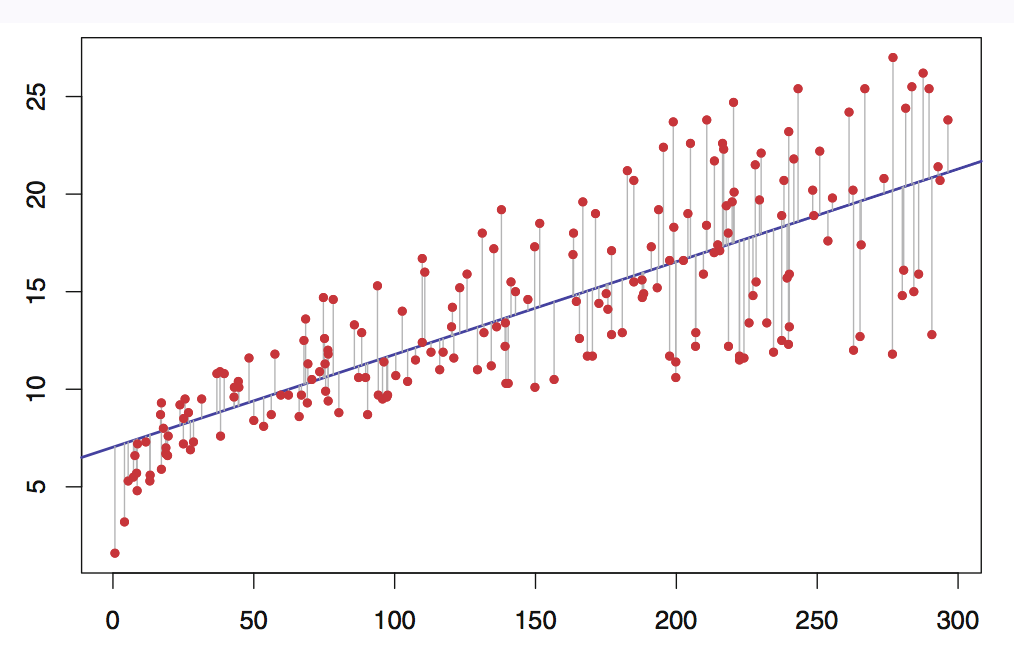
\includegraphics{regression.png}
\caption{Linear Regression - Least Squares}
\end{figure}

\begin{verbatim}
## [1] 84.03009
\end{verbatim}

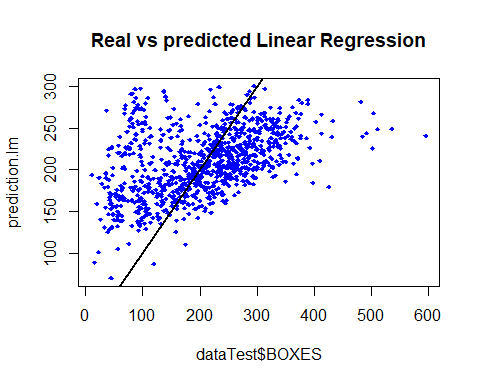
\includegraphics{Ed_Demo_files/figure-latex/unnamed-chunk-4-1.pdf}

\section{Create the decision tree
model}\label{create-the-decision-tree-model}

\begin{Shaded}
\begin{Highlighting}[]
\NormalTok{model.dt <-}\StringTok{ }\KeywordTok{rpart}\NormalTok{(data_formula_boxes, }\DataTypeTok{method =} \StringTok{"anova"}\NormalTok{, }\DataTypeTok{data=}\NormalTok{dataTrain)}
\NormalTok{prediction.dt <-}\StringTok{ }\KeywordTok{predict}\NormalTok{(model.dt, }\DataTypeTok{newdata =}\NormalTok{ dataTest)}
\NormalTok{rmse.dt <-}\StringTok{ }\KeywordTok{sqrt}\NormalTok{(}\KeywordTok{mean}\NormalTok{((dataTest}\OperatorTok{$}\NormalTok{BOXES}\OperatorTok{-}\NormalTok{prediction.dt)}\OperatorTok{^}\DecValTok{2}\NormalTok{))}
\NormalTok{rmse.dt}
\end{Highlighting}
\end{Shaded}

\begin{verbatim}
## [1] 54.70869
\end{verbatim}

\begin{Shaded}
\begin{Highlighting}[]
\KeywordTok{plot}\NormalTok{(dataTest}\OperatorTok{$}\NormalTok{BOXES,prediction.dt,}\DataTypeTok{col=}\StringTok{'blue'}\NormalTok{,}\DataTypeTok{main=}\StringTok{'Real vs predicted Decision Tree'}\NormalTok{,}\DataTypeTok{pch=}\DecValTok{18}\NormalTok{, }\DataTypeTok{cex=}\FloatTok{0.7}\NormalTok{)}
\KeywordTok{abline}\NormalTok{(}\DecValTok{0}\NormalTok{,}\DecValTok{1}\NormalTok{,}\DataTypeTok{lwd=}\DecValTok{2}\NormalTok{)}
\end{Highlighting}
\end{Shaded}

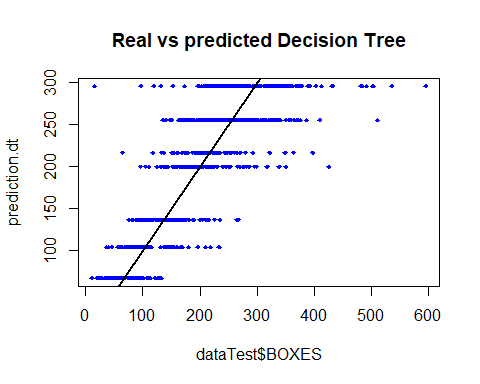
\includegraphics{Ed_Demo_files/figure-latex/unnamed-chunk-5-1.pdf}

\section{Create the random forest
model}\label{create-the-random-forest-model}

\begin{Shaded}
\begin{Highlighting}[]
\NormalTok{dataTrain_fac <-}\StringTok{ }\NormalTok{dataTrain }\OperatorTok\StringTok{ }\KeywordTok{mutate_if}\NormalTok{(is.character, as.factor)}
\NormalTok{dataTest_fac <-}\StringTok{ }\NormalTok{dataTest }\OperatorTok\StringTok{ }\KeywordTok{mutate_if}\NormalTok{(is.character, as.factor)}
\NormalTok{model.rf <-}\StringTok{ }\KeywordTok{randomForest}\NormalTok{(data_formula_boxes, }\DataTypeTok{data =}\NormalTok{ dataTrain_fac)}
\NormalTok{prediction.rf <-}\StringTok{ }\KeywordTok{predict}\NormalTok{(model.rf, }\DataTypeTok{newdata =}\NormalTok{ dataTest_fac)}
\NormalTok{rmse.rf <-}\StringTok{ }\KeywordTok{sqrt}\NormalTok{(}\KeywordTok{mean}\NormalTok{((dataTest_fac}\OperatorTok{$}\NormalTok{BOXES}\OperatorTok{-}\NormalTok{prediction.rf)}\OperatorTok{^}\DecValTok{2}\NormalTok{))}
\NormalTok{rmse.rf}
\end{Highlighting}
\end{Shaded}

\begin{verbatim}
## [1] 46.32067
\end{verbatim}

\begin{Shaded}
\begin{Highlighting}[]
\KeywordTok{plot}\NormalTok{(dataTest}\OperatorTok{$}\NormalTok{BOXES,prediction.rf,}\DataTypeTok{col=}\StringTok{'blue'}\NormalTok{,}\DataTypeTok{main=}\StringTok{'Real vs predicted Random Forest'}\NormalTok{,}\DataTypeTok{pch=}\DecValTok{18}\NormalTok{, }\DataTypeTok{cex=}\FloatTok{0.7}\NormalTok{)}
\KeywordTok{abline}\NormalTok{(}\DecValTok{0}\NormalTok{,}\DecValTok{1}\NormalTok{,}\DataTypeTok{lwd=}\DecValTok{2}\NormalTok{)}
\end{Highlighting}
\end{Shaded}

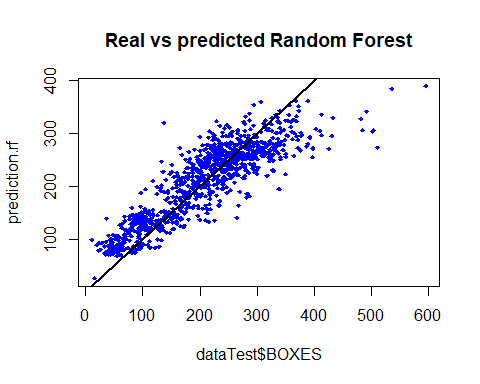
\includegraphics{Ed_Demo_files/figure-latex/unnamed-chunk-6-1.pdf}

\section{\texorpdfstring{Create the neural net model \textbf{\emph{Clean
up the code to match the other
chunks}}}{Create the neural net model Clean up the code to match the other chunks}}\label{create-the-neural-net-model-clean-up-the-code-to-match-the-other-chunks}

\begin{Shaded}
\begin{Highlighting}[]
\KeywordTok{library}\NormalTok{(}\StringTok{'neuralnet'}\NormalTok{)}

\NormalTok{maxs <-}\StringTok{ }\KeywordTok{apply}\NormalTok{(dataTrain, }\DecValTok{2}\NormalTok{, max)}
\NormalTok{mins <-}\StringTok{ }\KeywordTok{apply}\NormalTok{(dataTrain, }\DecValTok{2}\NormalTok{, min)}
\NormalTok{scaled_train <-}\StringTok{ }\KeywordTok{as.data.frame}\NormalTok{(}\KeywordTok{scale}\NormalTok{(dataTrain, }\DataTypeTok{center =}\NormalTok{ mins, }\DataTypeTok{scale =}\NormalTok{ maxs }\OperatorTok{-}\StringTok{ }\NormalTok{mins))}
\NormalTok{scaled_test <-}\StringTok{ }\KeywordTok{as.data.frame}\NormalTok{(}\KeywordTok{scale}\NormalTok{(dataTest, }\DataTypeTok{center =}\NormalTok{ mins, }\DataTypeTok{scale =}\NormalTok{ maxs }\OperatorTok{-}\StringTok{ }\NormalTok{mins))}
\NormalTok{n <-}\StringTok{ }\KeywordTok{names}\NormalTok{(scaled_train)}
\NormalTok{f <-}\StringTok{ }\KeywordTok{as.formula}\NormalTok{(}\KeywordTok{paste}\NormalTok{(}\StringTok{"BOXES ~"}\NormalTok{, }\KeywordTok{paste}\NormalTok{(n[}\OperatorTok{!}\NormalTok{n }\OperatorTok\StringTok{ "BOXES"}\NormalTok{], }\DataTypeTok{collapse =} \StringTok{" + "}\NormalTok{)))}

\NormalTok{nn <-}\StringTok{ }\KeywordTok{neuralnet}\NormalTok{(f,}\DataTypeTok{data=}\NormalTok{scaled_train,}\DataTypeTok{hidden=}\KeywordTok{c}\NormalTok{(}\DecValTok{8}\NormalTok{,}\DecValTok{4}\NormalTok{),}\DataTypeTok{linear.output=}\NormalTok{F)}
\NormalTok{pr.nn <-}\StringTok{ }\KeywordTok{compute}\NormalTok{(nn,scaled_test[,}\DecValTok{0}\OperatorTok{:}\DecValTok{11}\NormalTok{])}
\NormalTok{pr.nn_ <-}\StringTok{ }\NormalTok{pr.nn}\OperatorTok{$}\NormalTok{net.result}\OperatorTok{*}\NormalTok{(}\KeywordTok{max}\NormalTok{(data}\OperatorTok{$}\NormalTok{BOXES)}\OperatorTok{-}\KeywordTok{min}\NormalTok{(data}\OperatorTok{$}\NormalTok{BOXES))}\OperatorTok{+}\KeywordTok{min}\NormalTok{(data}\OperatorTok{$}\NormalTok{BOXES)}
\NormalTok{test.r <-}\StringTok{ }\NormalTok{(scaled_test}\OperatorTok{$}\NormalTok{BOXES)}\OperatorTok{*}\NormalTok{(}\KeywordTok{max}\NormalTok{(data}\OperatorTok{$}\NormalTok{BOXES)}\OperatorTok{-}\KeywordTok{min}\NormalTok{(data}\OperatorTok{$}\NormalTok{BOXES))}\OperatorTok{+}\KeywordTok{min}\NormalTok{(data}\OperatorTok{$}\NormalTok{BOXES)}
\NormalTok{rmse.nn <-}\StringTok{ }\KeywordTok{sqrt}\NormalTok{(}\KeywordTok{mean}\NormalTok{((dataTest}\OperatorTok{$}\NormalTok{BOXES}\OperatorTok{-}\NormalTok{pr.nn_)}\OperatorTok{^}\DecValTok{2}\NormalTok{))}
\NormalTok{rmse.nn}
\end{Highlighting}
\end{Shaded}

\begin{verbatim}
## [1] 51.01262684
\end{verbatim}

\begin{Shaded}
\begin{Highlighting}[]
 \KeywordTok{plot}\NormalTok{(dataTest}\OperatorTok{$}\NormalTok{BOXES,pr.nn_,}\DataTypeTok{col=}\StringTok{'blue'}\NormalTok{,}\DataTypeTok{main=}\StringTok{'Real vs predicted Neural Net'}\NormalTok{,}\DataTypeTok{pch=}\DecValTok{18}\NormalTok{, }\DataTypeTok{cex=}\FloatTok{0.7}\NormalTok{)}
 \KeywordTok{abline}\NormalTok{(}\DecValTok{0}\NormalTok{,}\DecValTok{1}\NormalTok{,}\DataTypeTok{lwd=}\DecValTok{2}\NormalTok{)}
\end{Highlighting}
\end{Shaded}

\includegraphics{Ed_Demo_files/figure-latex/unnamed-chunk-7-1.pdf}

\section{Create the boosted random forest
model}\label{create-the-boosted-random-forest-model}

\begin{Shaded}
\begin{Highlighting}[]
\KeywordTok{tic}\NormalTok{()}
\NormalTok{model.xgb <-}\StringTok{ }\KeywordTok{xgb.train}\NormalTok{(}\DataTypeTok{data=}\NormalTok{xgTrain_box, }\DataTypeTok{objective=}\StringTok{'reg:linear'}\NormalTok{, }\DataTypeTok{eval_metric=}\StringTok{'rmse'}\NormalTok{, }\DataTypeTok{booster=}\StringTok{'gbtree'}\NormalTok{, }\DataTypeTok{watchlist =} \KeywordTok{list}\NormalTok{(}\DataTypeTok{train=}\NormalTok{xgTrain_box, }\DataTypeTok{validate=}\NormalTok{xgVal_box), }
                  \DataTypeTok{early_stopping_rounds=}\DecValTok{100}\NormalTok{, }\DataTypeTok{nrounds =} \DecValTok{100000}\NormalTok{, }\DataTypeTok{num_parallel_tree=}\DecValTok{20}\NormalTok{, }\DataTypeTok{print_every_n =} \DecValTok{20}\NormalTok{, }\DataTypeTok{nthread=}\DecValTok{8}\NormalTok{,}\DataTypeTok{eta =}\NormalTok{ .}\DecValTok{1}\NormalTok{, }\DataTypeTok{max_depth =} \DecValTok{7}\NormalTok{)}
\end{Highlighting}
\end{Shaded}

\begin{verbatim}
## [1]  train-rmse:206.662491   validate-rmse:206.324921 
## Multiple eval metrics are present. Will use validate_rmse for early stopping.
## Will train until validate_rmse hasn't improved in 100 rounds.
## 
## [21] train-rmse:49.004692    validate-rmse:51.825565 
## [41] train-rmse:37.739918    validate-rmse:44.912476 
## [61] train-rmse:34.274696    validate-rmse:44.728710 
## [81] train-rmse:32.041958    validate-rmse:45.088673 
## [101]    train-rmse:30.619726    validate-rmse:45.431015 
## [121]    train-rmse:28.945339    validate-rmse:45.697258 
## [141]    train-rmse:27.396843    validate-rmse:46.126431 
## Stopping. Best iteration:
## [55] train-rmse:35.154510    validate-rmse:44.669308
\end{verbatim}

\begin{Shaded}
\begin{Highlighting}[]
\KeywordTok{toc}\NormalTok{()}
\end{Highlighting}
\end{Shaded}

\begin{verbatim}
## 37.64 sec elapsed
\end{verbatim}

\begin{Shaded}
\begin{Highlighting}[]
\NormalTok{dataTest.xgb <-}\StringTok{ }\KeywordTok{build.x}\NormalTok{(data_formula_boxes, }\DataTypeTok{data=}\NormalTok{dataTest, }\DataTypeTok{contrasts =} \OtherTok{FALSE}\NormalTok{, }\DataTypeTok{sparse =} \OtherTok{TRUE}\NormalTok{)}

\NormalTok{prediction.xgb <-}\StringTok{ }\KeywordTok{predict}\NormalTok{(model.xgb, }\DataTypeTok{newdata =}\NormalTok{ dataTest.xgb)}
\KeywordTok{plot}\NormalTok{(dataTest}\OperatorTok{$}\NormalTok{BOXES,prediction.xgb,}\DataTypeTok{col=}\StringTok{'blue'}\NormalTok{,}\DataTypeTok{main=}\StringTok{'Real vs predicted Boosted Forest'}\NormalTok{,}\DataTypeTok{pch=}\DecValTok{18}\NormalTok{, }\DataTypeTok{cex=}\FloatTok{0.7}\NormalTok{)}
 \KeywordTok{abline}\NormalTok{(}\DecValTok{0}\NormalTok{,}\DecValTok{1}\NormalTok{,}\DataTypeTok{lwd=}\DecValTok{2}\NormalTok{)}
\end{Highlighting}
\end{Shaded}

\includegraphics{Ed_Demo_files/figure-latex/unnamed-chunk-8-1.pdf}


\end{document}
